
\section{Results}

The model was tested in several scenarios. First, the price 
dynamics and order book evolution are studied with a simple one market settings in which the dividend
yield and interest rate are set to zero. Then the same aspects are investigated
using more complex settings: only some of the traders are allowed to place orders
per trading session and the dividend yield and interest rate are set to random walk.
Then arbitrage is studied using 
a setting in which there exists two identical markets.


\subsection{Single asset simulation}
% Price dynamics, stylized facts, order book evolution
The single asset simulation was run twice: first run
was conducted with a starting market price of 500 and second
with a starting market price of 1500. The simulations were
run with 500 traders trading 1000 rounds. The 
amount of currency and the amount of stock 
a trader owns in the beginning of the simulation were set to
10 000 000 and 10 000 respectively. Therefore
the ratio of stock to currency is 1 000 which
is the expected equilibrium price as there are
no payouts in either asset. The amount of currency
per trader may seem much but as the tick size is one,
it may be more convenient to think the currency in amounts
in cents or pennies. The standard deviation of
the price each trader bids and asks with is set to 20. The 
starting market price was set to 400 to study the 

% Descriptive analysis
The evolution of trade prices, quantities and values thorough
the trading sessions for both simulations are shown in the figure
~\ref{fig:basic_trades}. As can be observed,
the near equilibrium market price is achieved in around 20 trading
sessions for both runs. The reason why the price stays slightly 
under the equilibrium price may be caused by the implementation of
determining the order price and order quantity. If a trader decides
to allocate less currency on an order than the decided order price 
the order gets obviously invalidated but there is no such
limitation for placing asks. Therefore there might be a slightly less
bids than asks in general. 

\begin{figure}
    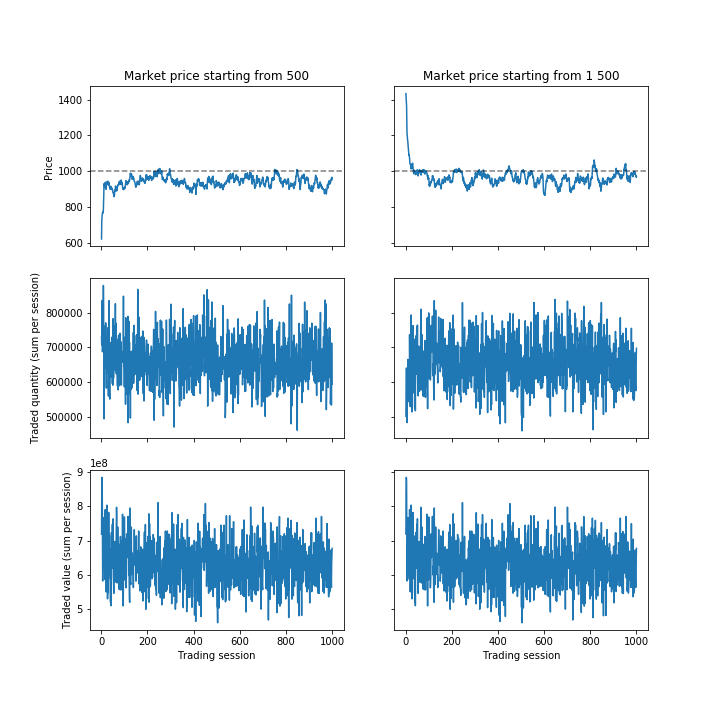
\includegraphics[width=\linewidth]{plots/basic_trades.png}
    \caption{Evolution of price and quantity}
    \label{fig:basic_trades}
\end{figure}

% How the market converged to equilibrium
The market depths shown in figure ~\ref{fig:market_depths} suggests that the
converge to equilibrium is caused by balancing the sides of the market. 
In the figure the order book is visualized for the first 100 trading sessions. 
The surface describes the evolution of the cumulative bids and cumulative asks 
thorough time and the bottom of the valley in the surface is the bid-ask spread. 
The left side from the valley is the the bid book and the right is the ask book. The 
ask side of the market is almost completely missing initially in the run that
starts with lower market price while the opposite is true for the run with higher
initial market price. The side emerges rapidly after few trading session
and the market price approaches near equilibrium price and vice versa for the 
simulation starting with higher market price.

\begin{figure}
    \centering
    \begin{subfigure}{.5\textwidth}
      \centering
      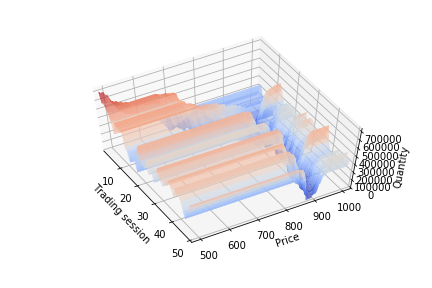
\includegraphics[width=\linewidth]{plots/basic_market_depth_converge_lower.png}
      \caption{Starting price 500}
      \label{fig:market_depth_lower}
    \end{subfigure}%
    \begin{subfigure}{.5\textwidth}
      \centering
      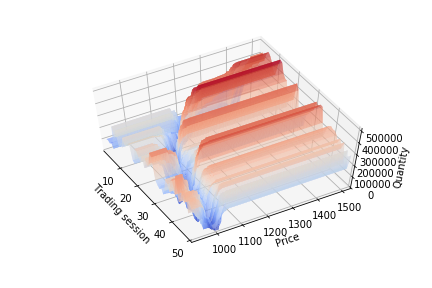
\includegraphics[width=\linewidth]{plots/basic_market_depth_converge_higher.png}
      \caption{Starting price 1 500}
      \label{fig:market_depth_higher}
    \end{subfigure}
    \caption{Converge of the order book to equilibrium}
    \label{fig:market_depths}
\end{figure}


% stylized facts
The stylized facts are also inline with the literature. There is no autocorrelation
in the relative changes in the market price as seen in figure n. In addition, with
current setup there are some volatility clusters with 10 trade window.


\subsection{Multi asset simulation}
